\section{Runner}
As stated in the \autoref{requirements} Requirements, the \textit{Runner} should be a piece of software enabling the user to run the automations created by the \textit{Editor} application.
During the implementation, only small changes were made to the initial design.

The \textit{Runner} is implemented as a \textit{Node.js} module and has been published as an \texttt{npm} package \texttt{@wbr-project/wbr-interpret@0.9.2}.
The user-friendly \textit{Runner} interface is a part of the \textit{Editor} application, as both tools together create a simple and easy-to-use environment for developing the web automations.

\subsection{Performance}

According to the nonfunctional requirement \textit{1.2.2.2.1}, the \textit{Runner} should implement the automation execution in an optimized way. 
While this requirement is rather vague, there are actually several ways the \textit{Runner} application tries to do so.

\subsubsection{Parallelization}

As mentioned in the \autoref{markov} Reactions, the workflow definition format is designed in such way that every step depends on the previous browser state only. 
This allows us to think of different browser tabs as of whole different environments \footnote{Only regarding the workflow execution, they still can share e.g. cookies.} 
and let the \textit{Runner} parallelize the automation between multiple tabs, possibly reducing the time required for the execution.

The \texttt{Interpreter} programmable interface allows the user to set maximum number of concurrent tabs.
Using the proper method of enqueuing links in the workflow (action \texttt{enqueueLinks}) protects the internal \textit{Runner} browser from opening too many tabs at once, which might hurt the performance.
The enqueued links are then opened as individual tabs by the \textit{Runner} with respect to the set concurrency.

In case a tab gets open e.g. as a popup window, it is not interacted with until the desired concurrency is reached.
However, accumulating multiple such tabs can still lead to performace degradation, as they still have to exist in the browser memory.

\subsubsection{Browser communication} \label{browsercom}
As mentioned in the \autoref{runnerDesign} Runner, the communication between the \textit{Interpreter} part of the \textit{Runner} and the internal web browser is facilitated using the \textit{Playwright} library.
While Playwright already provides an optimized way of communication with the browser using the \acs{CDP} protocol and alternatives, the text-based interprocess communication still poses a certain performance bottleneck.

While designing the \textit{Runner}, it was a priority to reduce the amount of calls to the \textit{Playwright} library, as pretty much any \textit{Playwright} call results in a \acs{CDP} message being sent.
During the condition matching phase of the workflow exection, the current browser state is fetched only once and the rule is then matched statically, instead of quering the browser repeatedly for the possible current URL, CSS selectors etc.

This is possible because of the simple design of the workflow definition format, allowing us to gather all the conditions statically. 
Knowing all the conditions, the full browser state can be then described by the truthiness/falsiness of those conditions, which is all that is needed for the decision making mechanism of the \textit{Interpreter} to choose the next step to take.

\subsection{Extra features}

On top of the features described in the \autoref{runnerDesign} Runner, there are some additional features implemented into the \textit{Runner} package.
While those features are tested and are available in the \verb|main| branch of the project, the other parts of the project - mainly the \textit{Editor} - typically does not provide full support.

\subsubsection{Workflow parametrization}

The \textit{Runner} module provides support for workflow parametrization. 
Any nonintegral part of the worklfow can be replaced with a special structure, for example like this:
\begin{lstlisting}[language=json]
    {
        ...
            "url": { $param: "address" },
        ...
    }
\end{lstlisting}

Before the workflow execution, the \textit{Runner} receives a dictionary of the parameters' values, replacing every \texttt{\{\$param\}} field with the declared value.
When initialized with value \texttt{\{"address" : "https://abc.xyz"\}}, the example above turns into

\begin{lstlisting}[language=json]
    {
        ...,
            "url": "https://abc.xyz",
        ...
    }
\end{lstlisting}

In case the user does not provide values for all the parameters or provides values for parameters non-existent in the workflow, the \textit{Runner} warns the user about this and does not continue with the workflow execution.

This feature can be utilized to create more universal workflow definitions, letting the end user to set certain parts of the workflow to match their use case.
The parametrized fields can be e.g. login credentials, URL of the page to run the automation on or a custom message or data to paste to the website.

\subsubsection{Automatic data extraction}

While the \textit{Runner} supports all the methods from the Playwright's \texttt{Page} class,
it also implements methods for automating data extraction from the browser.

The \texttt{scrape} method allows the user to extract data from the current page by utilizing an algorithm 
looking for the ``important'' data in the page. The user can restrict the search to a specific element subtree
by passing the selector of the root element as the only argument to this method.

The ``importance'' of the data in the page is determined using multiple heuristics, mostly by looking for 
similar-sized elements with similar content - these are believed to be the ``scrapable'' data - e.g. online store product cards, rows of a table, etc.

\subsubsection{Guided data extraction}

The \texttt{scrapeSchema} method acts as a guided counterpart of the \texttt{scrape} method.
By specifying the names of columns and their respective selectors in the only argument of this method, 
the \textit{Runner} extracts data from these selectors, and stores them in a dictionary, where the keys are the column names.

In case the selectors target multiple elements on the same page, the \textit{Runner} will group the extracted data and output multiple dictionaries.
If the numbers of the targetted elements do not match across the columns, the \textit{Runner} tries to group the data by the \acs{DOM} hierarchy in the web page, possibly leaving some output fields empty.

Here follows an example of the \texttt{scrapeSchema} method usage and the logic behind it.

\begin{figure}[!h]
    \begin{center}
        \fbox{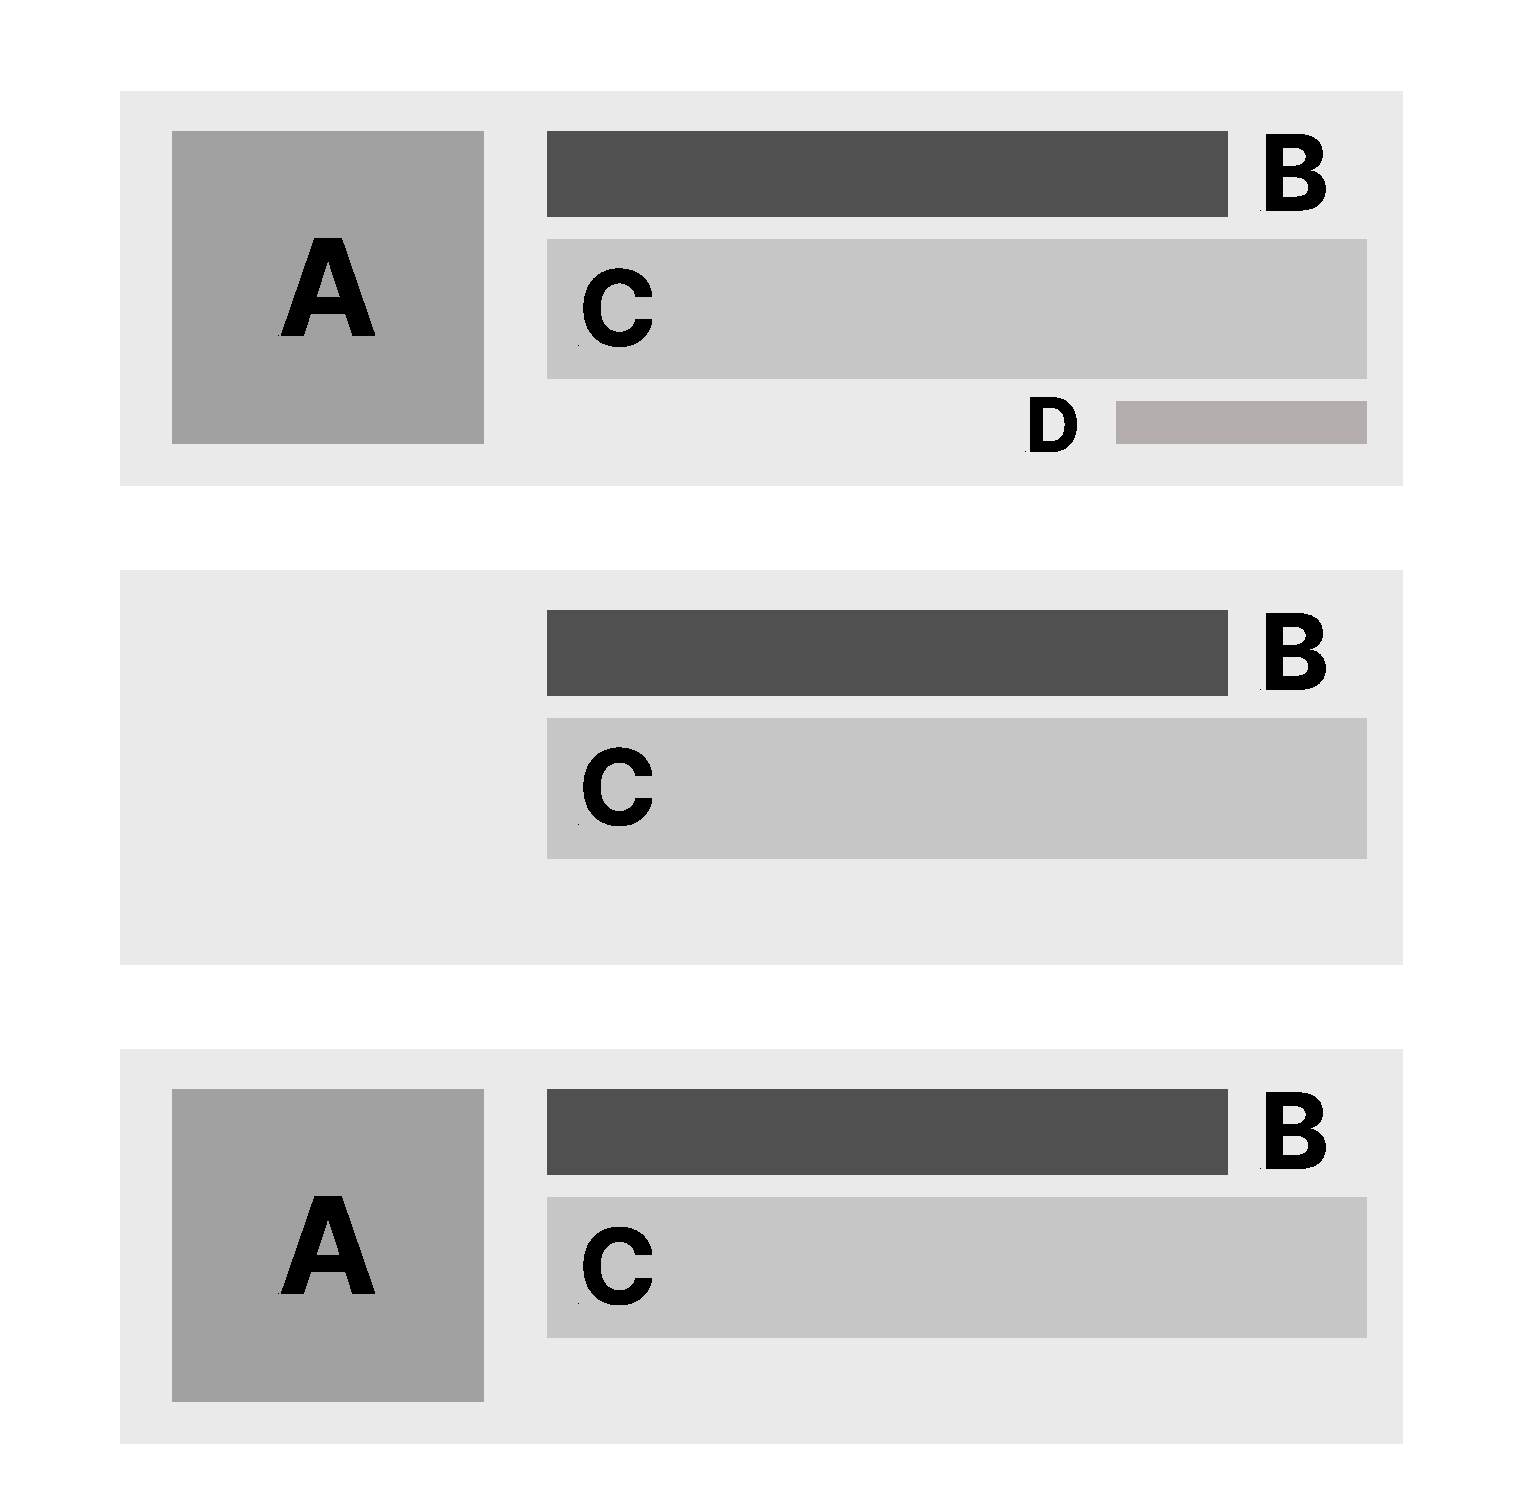
\includegraphics[width=0.4\textwidth]{./img/algos/scrapeSchema.pdf}}
    \end{center}
    \caption{Example page to be scraped}\label{scrapeSchema}
\end{figure}

The \autoref{scrapeSchema} shows an example page containing a table of user profiles. 
A user card can contain a \textit{photo of the user} (A), their \textit{name} (B), their \textit{profile description} (C) and their \textit{phone number} (D).
The letters represent the selectors for the \textit{Runner} to extract the data from.

The user provides the \texttt{scrapeSchema} method with the following schema:
    \begin{lstlisting}[language=json]
                {
                    "photo": "A",
                    "name":  "B",
                    "desc":  "C",
                    "phone": "D"
                }
    \end{lstlisting}

The \textit{Runner} extracts the data from the page. The data is stored in an array of dictionaries, where each dictionary corresponds to a user card.

\begin{lstlisting}[language=json]
[
    {
        "photo": "https://abc.xyz/img/user123.jpg",
        "name":  "John Doe",
        "desc":  "Lorem ipsum dolor sit...",
        "phone": "123-456-7890"
    },
    {
        "photo": undefined,
        "name":  "Mark Smith",
        "desc":  "Ipsum dolor amet sit...",
        "phone": undefined
    },
    {
        "photo": "https://abc.xyz/img/user234.jpg",
        "name":  "Jane Green",
        "desc":  "Sit dolor ipsum lorem...",
        "phone": undefined
    },
]
\end{lstlisting}

Note how the contents of the corresponding elements are paired, leaving the missing fields empty.
This is done by traversing the \acs{DOM} tree of the page, and grouping the elements by their common parents.